\documentclass[a4paper, 12pt, titlepage]{article}
\setlength{\oddsidemargin}{0in} \setlength{\evensidemargin}{0in}
\setlength{\textwidth}{6.2in}
\setlength{\topmargin}{-0.2in} \setlength{\textheight}{8.8in}

\usepackage{graphicx}
\graphicspath{ {/home/michal/development/workspace/CS12320_assign2/doc/img/} }

\title{Individual Assignment: Patience is a Virtue}
\author{Michal Wojciech Goly [mwg2]}
\date{1st May 2015}

\begin{document}

\maketitle
\tableofcontents
\newpage

\section{Introduction}
\subsection{Project description}
Patience is a simple card game for one player, in which the objective is to end up with 
one pile of cards on the table. There are 52 playing cards at the start of the game, all
facing downwards in a pack. Player can then deal a card which will be removed from the
deck and put on the table facing upwards. By continuing to do so, there could potentially
be 52 cards on the table all facing upwards, unless a move was made. Apart from dealing
cards there are two additional valid moves in the game. You can join two cards 
together if they have the same suit or value and if:
\begin{itemize}
	\item They are next to each other
	\item There are two other cards between them
\end{itemize}
When joined, the card further to the right will be placed on top of the other, regardless
of the order in which they have been selected. Each move is worth 10 points in the game. 
Therefore because there are 51 available moves in total, the highest possible score is
510 points. 

\subsection{Game controls} 
Because the user interface is fully graphical, to play the game user can simply click on 
the cards. For example if the player wants to deal a card, he should click on the pack 
and a move will be made. Similarly, to select a card user has to click on it. In order to
indicate which card was selected, a blue border will be painted around it.

Additional options are available within the button panel at the bottom of the window. 
Player can display contents of the pack, as well as shuffle it. Second option is only
permitted once and should typically be selected at the start of the game. Pack is not 
randomized by default due to the requirements specification of the assignment. Last two
options allow an automation of the gameplay. Player can either make use of the 'Play for
me once' option which as expected will make one valid move in the game, if there is one,
or specify the amount of moves to be made by clicking the 'Play for me x times' button.

Game ends either if the automation algorithm detects that there are no more moves 
available, user presses the 'x' exit button on the top of the window or game is won.
Before the application closes, a smaller window will pop up to ask the player to enter
his name in order to save his score. User can choose not to store his result by leaving
the name field blank.

\newpage

\section{Requirements Analysis}
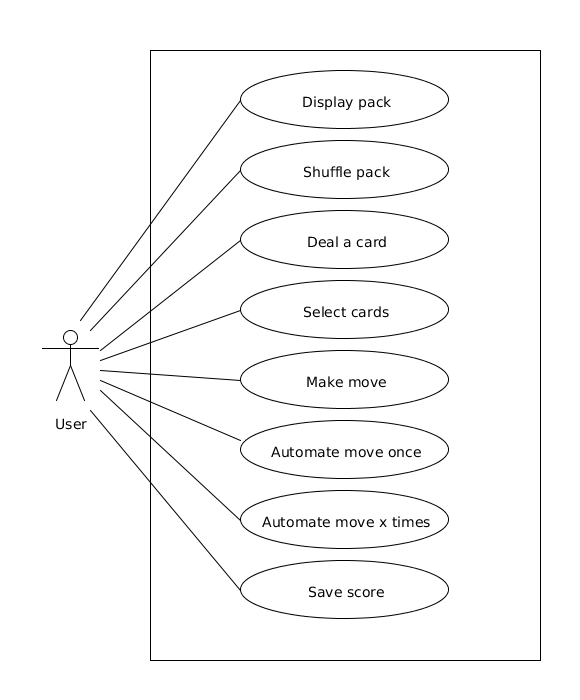
\includegraphics[width=\textwidth]{useDiagram}

\section{Design}
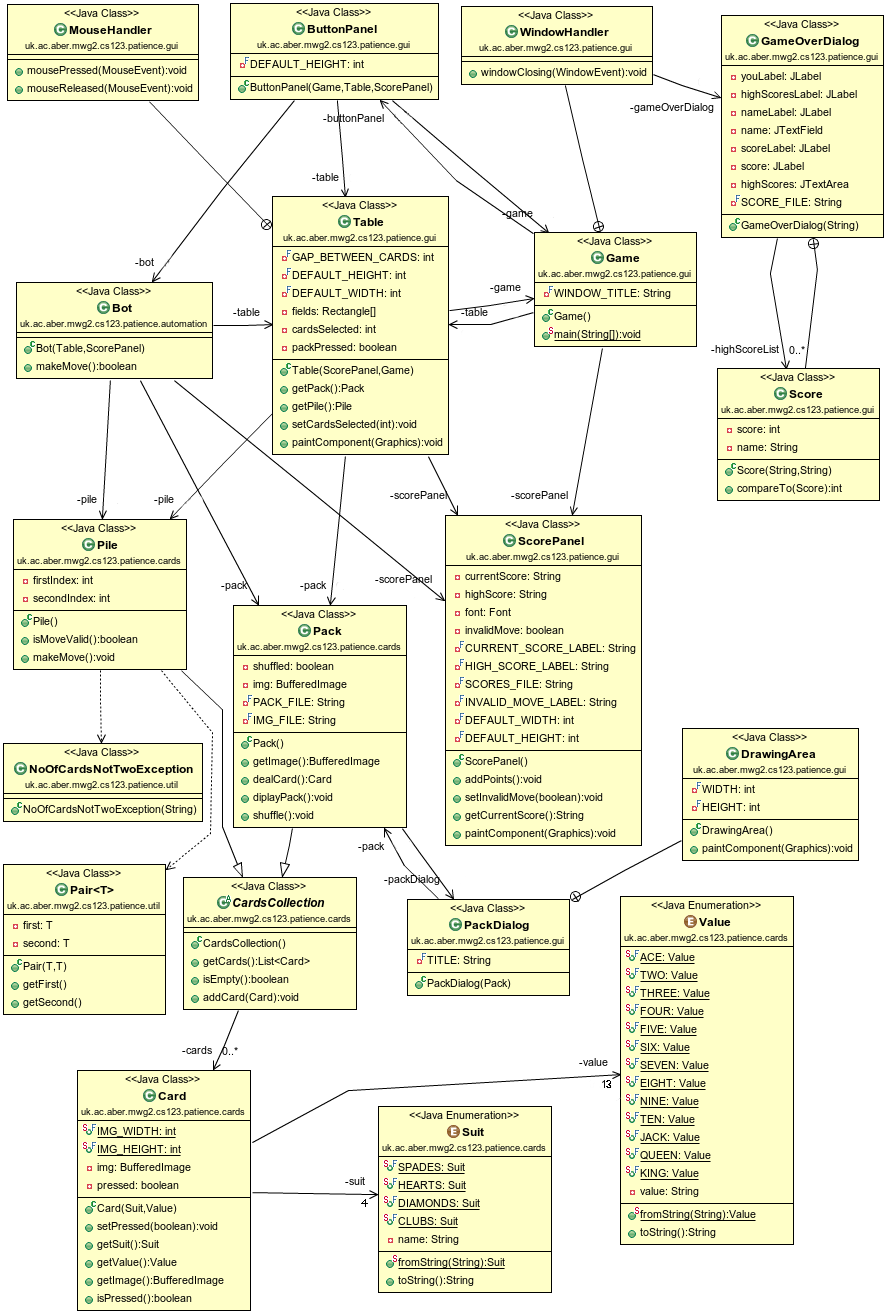
\includegraphics[width=\textwidth]{classDiagram}

\section{Testing}

\section{Evaluation}

\end{document}
